\subsection{Simulator validation}\label{sec:validation}
\paragraph{Gokmen and Haensch 2020.} We map their RPU-baseline device onto our model:
\begin{itemize}
\item step $10^{-3}$ at $w=0$;
\item mean saturation slope $1.66$ with a 25\% per-device spread;
\item 30\% step spread and 30\% cycle-to-cycle noise;
\item a symmetry point at $w=0$ for every device.
\end{itemize}
We train their 784--256--128--10 sigmoid network on MNIST for 50 epochs at their learning rate of 0.01. The results are in
Table~\ref{tab:e1} and Fig.~\ref{fig:validation}a.
\begin{itemize}
\item FP reaches \REOneFpErr\% test error, against their 2.0\%.
\item SGD on the device reaches \REOneSgdErr\% [\REOneSgdLo, \REOneSgdHi], against ``about 15\%''.
\item Tiki-Taka reaches \REOneTtvOneErr\% [\REOneTtvOneLo, \REOneTtvOneHi], against ``close to 2\%''.
\end{itemize}
By our pre-registered criteria the agreement is \textbf{\REOneVerdict}: this is agreement with selected published outcomes
under a simplified read model, not a full quantitative validation. Matching an endpoint under different sources of error cannot
rule out compensating differences, and the batch-64 result below shows how sensitive the SGD arm is to the protocol. These
validation runs used the original simulator (TTv1 has no reset, so the reset repair does not touch them). The known
differences are listed in Section~\ref{sec:limits}:
\begin{itemize}
\item we use mini-batches of 16, not 1;
\item we do not model read noise, ADC/DAC quantisation or analog biases.
\end{itemize}
At batch 64 the FP and TTv1 results barely move, but SGD on the device degrades further. Summing more samples' pulses before the
weight changes hurts a strongly asymmetric device, which is another reason to use batch 16 as the closer match to their batch 1.

\paragraph{Rasch et al.\ 2024, qualitatively.} We use a 20-state soft-bounds device with an uncorrected reference offset of
$\sigma_r=0.5$ (Table~\ref{tab:e1b}, Fig.~\ref{fig:validation}b).
\begin{itemize}
\item TTv2's test error rises from \REOnebTtvTwoSrZero\% to \REOnebTtvTwoSrFive\%.
\item c-TTv2 rises less, from \REOnebCttvTwoSrZero\% to \REOnebCttvTwoSrFive\%.
\item AGAD is unaffected: \REOnebAgadSrZero\% versus \REOnebAgadSrFive\%.
\end{itemize}
This is the published ordering; our pre-registered check reads \textbf{\REOnebVerdict}. It rests on two seeds per condition
and an ordering, so it does not establish that our c-TTv2 and AGAD are equivalent to the published implementations, and the
absence of a detected change does not show that AGAD is unaffected. In our implementation AGAD starts from a higher error at
zero offset on this very coarse device.

\paragraph{The device presets against AIHWKIT itself (revision).} On a rented machine (never on our desk) we installed AIHWKIT
\RVaihwVersion{} from PyPI and drove its EcRamPresetDevice and EcRamMOPresetDevice through long up, down and alternating pulse
schedules (500 devices each, with and without cycle-to-cycle noise), using its own plotting utilities. Our AIHWKIT-mode tile,
driven through the same schedules, \RVaihwVerdict{} (largest mean difference \RVaihwLiMaxDiff{} for Li-ECRAM and
\RVaihwMoMaxDiff{} for MO-ECRAM, in weight units; the pre-registered tolerance is $\max(4\,\mathrm{SE},2\,\Delta w_{\min})$ at every
stored pulse). The original field-copy mapping differs by up to \RVaihwLiOldMaxDiff{} for Li-ECRAM, mostly at the bounds
(Appendix~\ref{app:revision}).

% generated by analyze.py (do not edit)
\begin{table}[t]\centering\small\caption{Validation against Gokmen and Haensch 2020 (FCN 784-256-128-10, MNIST, 50 epochs): test error in \%, our mean and 95\% interval over 3 seeds at batch 16, and one seed at batch 64.}\label{tab:e1}
\fitbox{\begin{tabular}{lccc}\toprule
Arm & Published~\cite{gokmen2020} & Ours (batch 16) & Ours (batch 64)\\\midrule
FP (exact update) & 2.0 & 1.78 [1.75, 1.81] & 1.79 (n=1)\\
SGD on the RPU-baseline device & about 15 & 14.47 [12.68, 16.26] & 24.32 (n=1)\\
Tiki-Taka (TTv1) & close to 2 & 2.26 [2.13, 2.39] & 2.07 (n=1)\\
TTv2 (ours, 16 columns per batch) & -- & 2.59 [2.42, 2.75] & not run\\
\bottomrule\end{tabular}}\end{table}

% generated by analyze.py (do not edit)
\begin{table}[t]\centering\small\caption{Qualitative check of Rasch et al.\ 2024 (Fig.~5): a 20-state soft-bounds device with an uncorrected reference offset $\sigma_r$; test error in \% (mean and 95 \% $t$ interval, $n=2$; 10 epochs). FP: 2.69 [0.47, 4.92].}\label{tab:e1b}
\fitbox{\begin{tabular}{lccc}\toprule Offset & TTv2 & c-TTv2 & AGAD\\\midrule
$\sigma_r=0$ & 4.12 [2.79, 5.46] & 4.29 [3.91, 4.67] & 8.47 [7.58, 9.36]\\
$\sigma_r=0.5$ & 24.27 [18.23, 30.30] & 13.02 [10.99, 15.05] & 7.88 [3.49, 12.26]\\
\bottomrule\end{tabular}}\end{table}

\begin{figure}[t]\centering
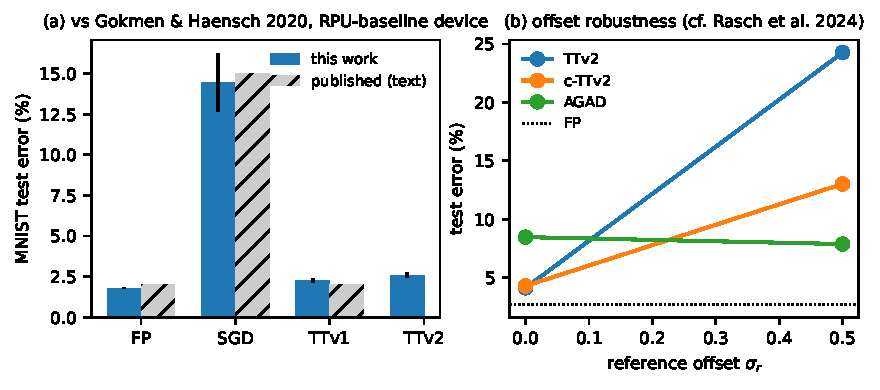
\includegraphics[width=\linewidth]{figs/fig_validation}
\caption{Simulator validation. (a) Test error of our simulator (mean and 95\% interval, 3 seeds) against the values stated in
the text of Gokmen and Haensch 2020 for their FCN on MNIST with the RPU-baseline device. (b) Robustness to an uncorrected
reference offset on a 20-state device (2 seeds), the qualitative trend of Rasch et al.\ 2024, Fig.~5.}\label{fig:validation}
\end{figure}
